\documentclass[]{article}
\usepackage{amsmath, amsfonts, amssymb, amsthm}
\usepackage{cancel}
\usepackage{pgfplots}
\usepackage{siunitx}
\usepackage[american]{circuitikz}
\usepackage{bm}
\usepackage{graphicx}
\usepackage{fullpage}
\usepackage{pdfpages}

\renewcommand{\thesection}{\arabic{section}}
\renewcommand{\thesubsection}{\thesection.\alph{subsection}}
\renewcommand{\thesubsubsection}{\thesubsection.\roman{subsubsection}}

\newtheorem{genthm}{Theorem}

\newcommand{\unit}[1]{\bm{\hat{#1}}}
\newcommand{\iprod}[2]{\left\langle #1, #2 \right\rangle}
\newcommand{\tpose}[1]{\left[#1\right]^{\! \top} \!\!}
\newcommand{\diff}[1]{\frac{d}{d #1}}

\title{EECS 16B HW10}
\author{Bryan Ngo}
\date{2020-04-12}

\begin{document}

\maketitle

\section{Frobenius Norm}

\begin{equation}
	\|\bm{A}\|_F = \sqrt{\sum_{i = 1}^N \sum_{j = 1}^N |\bm{A}_{ij}|^2}
\end{equation}

\subsection{}

\begin{genthm}
Given some matrix \(\bm{A}\),
\begin{equation}
	\|\bm{A}\|_F = \sqrt{\operatorname{tr}\{\tpose{\bm{A}} \bm{A}\}}
\end{equation}
where \(\operatorname{tr}\{\bm{A}\}\) is the trace operator
\begin{equation}
	\operatorname{tr}\{\bm{A}\} = \sum_{i = 1}^N \bm{A}_{ii}
\end{equation}
\end{genthm}

\begin{proof}
Examining \(\tpose{\bm{A}} \bm{A}\),
\begin{equation}
	\tpose{\bm{A}} \bm{A} =
	\begin{bmatrix}
	\tpose{\bm{a}_1} \\
	\tpose{\bm{a}_2} \\
	\vdots \\
	\tpose{\bm{a}_N}
	\end{bmatrix}
	\begin{bmatrix}
	\bm{a}_1 & \bm{a}_2 & \cdots & \bm{a}_N
	\end{bmatrix} =
	\begin{bmatrix}
	\iprod{\bm{a}_1}{\bm{a}_1} & \iprod{\bm{a}_1}{\bm{a}_2} & \cdots & \iprod{\bm{a}_1}{\bm{a}_N} \\
	\iprod{\bm{a}_2}{\bm{a}_1} & \iprod{\bm{a}_2}{\bm{a}_2} & \cdots & \iprod{\bm{a}_2}{\bm{a}_N} \\
	\vdots & \vdots & \ddots & \vdots \\
	\iprod{\bm{a}_N}{\bm{a}_1} & \iprod{\bm{a}_N}{\bm{a}_2} & \cdots & \iprod{\bm{a}_N}{\bm{a}_N}
	\end{bmatrix}
\end{equation}
where \(\bm{a}_i\) is a column vector of \(\bm{A}\).
Thus, the trace is
\begin{align}
	\operatorname{tr}\{\tpose{\bm{A}} \bm{A}\} &= \sum_{i = 1}^N \|\bm{a}_i\|^2 = \sum_{i = 1}^N \sum_{j = 1}^N \bm{A}_{ij}^2 \\
	\sqrt{\operatorname{tr}\{\tpose{\bm{A}} \bm{A}\}} &= \sqrt{\sum_{i = 1}^N \sum_{j = 1}^N \bm{A}_{ij}^2} = \|\bm{A}\|_F
\end{align}
\end{proof}

\subsection{}

\begin{genthm}
Given orthonormal matrices \(\bm{U}, \bm{V}\),
\begin{equation}
	\|\bm{UA}\|_F = \|\bm{AV}\|_F = \|\bm{A}\|_F
\end{equation}
\end{genthm}

\begin{proof}
Examining \(\bm{UA}, \bm{AV}\),
\begin{align}
	\bm{UA} &=
	\bm{U} \begin{bmatrix}
	\bm{a}_1 & \bm{a}_2 & \cdots & \bm{a}_N
	\end{bmatrix} =
	\begin{bmatrix}
	\bm{Ua}_1 & \bm{Ua}_2 & \cdots & \bm{Ua}_N
	\end{bmatrix} \\
	\bm{AV} &=
	\begin{bmatrix}
	\bm{a}'_1 \bm{V} \\
	\bm{a}'_2 \bm{V} \\
	\vdots \\
	\bm{a}'_N \bm{V}
	\end{bmatrix}
\end{align}
where \(\bm{a}_i\) is a column vector and \(\bm{a}'_i\) is a row vector.
Using \textbf{Equation 6},
\begin{equation}
	\|\bm{UA}\|_F = \sqrt{\sum_{i = 1}^N \|\bm{Ua}_i\|^2}
\end{equation}
Since linear transformations by orthonormal matrices do not change the norm of a vector,
\begin{equation}
	\sqrt{\sum_{i = 1}^N \|\bm{Ua}_i\|^2} = \sqrt{\sum_{i = 1}^N \|\bm{a}_i\|^2} = \|\bm{A}\|_F
\end{equation}
For the \(\bm{AV}\) case, we need only prove that \(\operatorname{tr}\{\tpose{\bm{AV}} \bm{AV}\} = \operatorname{tr}\{\tpose{\bm{A}} \bm{A}\}\),
\begin{align}
	\tpose{\bm{AV}} \bm{AV} &=
	\begin{bmatrix}
	\tpose{\bm{a}'_1 \bm{V}} & \tpose{\bm{a}'_2 \bm{V}} & \cdots & \tpose{\bm{a}'_N \bm{V}}
	\end{bmatrix}
	\begin{bmatrix}
	\bm{a}'_1 \bm{V} \\
	\bm{a}'_2 \bm{V} \\
	\vdots \\
	\bm{a}'_N \bm{V}
	\end{bmatrix} \\
	&= \sum_{i = 1}^N \tpose{\bm{a}'_i \bm{V}} \bm{a}'_i \bm{V} = \sum_{i = 1}^N \tpose{\bm{V}} \tpose{\bm{a}'} \bm{a}'_i \bm{V} = \sum_{i = 1}^N \|\bm{a}_i\|^2  \cancelto{\bm{I}}{\tpose{\bm{V}} \bm{V}} = \sum_{i = 1}^N \|\bm{a}_i\|^2
\end{align}
Thus, the trace is the same.
By \textbf{Equation 6}, so are their Frobenius norms.
\end{proof}

\subsection{}

\begin{genthm}
Given a matrix \(\bm{A} \in \mathbb{R}^{m \times n}\),
\begin{equation}
	\|\bm{A}\|_F = \sqrt{\sum_{i = 1}^N \sigma^2_i}
\end{equation}
where \(\sigma_i\) are the singular values of \(\bm{A}\).
\end{genthm}

\begin{proof}
Using the compact SVD, we can represent \(\bm{A} = \bm{US} \tpose{\bm{V}}\), where \(\bm{U}, \bm{V}\) are orthonormal matrices and \(\bm{S}\) is a diagonal matrix composed of the non-zero singular values.
If we leverage the fact that left \emph{and} right multiplication by orthonormal matrices does not change the Frobenius norm, we can simply reduce it to
\begin{equation}
	\|\bm{A}\|_F = \|\bm{US} \tpose{\bm{V}}\|_F = \|\bm{S}\|_F
\end{equation}
Since \(\bm{S}\) is a diagonal matrix, we use \textbf{Equation 6},
\begin{equation}
	\|\bm{S}\|_F = \sqrt{\sum_{i = 1}^N \|\bm{s}_i\|^2} = \sqrt{\sum_{i = 1}^N \sigma^2_i}
\end{equation}
where the last equality holds because \(\|\bm{s}_i\| = \sigma_i\) due to the diagonality of \(\bm{S}\).
\end{proof}

\section{Minimum Energy Control}

\begin{equation}
	\bm{x}[t + 1] = \begin{bmatrix}
	1 & 1 \\
	0 & 1
	\end{bmatrix} \bm{x}[t] + \begin{bmatrix}
	0 \\
	1
	\end{bmatrix} u[t]
\end{equation}

\subsection{}

We construct the controllability matrix for \(n = 5\),
\begin{align}
	\bm{C} &= \begin{bmatrix}
	\bm{b} & \bm{Ab} & \cdots & \bm{A}^{n - 1} \bm{b}
	\end{bmatrix} \\
	&= \begin{bmatrix}
	0 & 1 & 2 & 3 & 4 \\
	1 & 1 & 1 & 1 & 1
	\end{bmatrix}
\end{align}
Thus, to reach the target state, we have
\begin{equation}
	\begin{bmatrix}
	0 & 1 & 2 & 3 & 4 \\
	1 & 1 & 1 & 1 & 1
	\end{bmatrix} \begin{bmatrix}
	u[0] \\
	u[1] \\
	u[2] \\
	u[3] \\
	u[4]
	\end{bmatrix} =
	\begin{bmatrix}
	1 \\
	0
	\end{bmatrix}
\end{equation}
We can use the minimum norm equation \(\unit{u} = \tpose{\bm{C}} (\bm{C} \tpose{\bm{C}})^{-1} \bm{x}_{tgt}\) to obtain
\begin{align}
	\bm{C} \tpose{\bm{C}} &=
	\begin{bmatrix}
	0 & 1 & 2 & 3 & 4 \\
	1 & 1 & 1 & 1 & 1
	\end{bmatrix}
	\begin{bmatrix}
	0 & 1 \\
	1 & 1 \\
	2 & 1 \\
	3 & 1 \\
	4 & 1
	\end{bmatrix} =
	\begin{bmatrix}
	30 & 10 \\
	10 & 5
	\end{bmatrix}
	\overset{-1}{\Longrightarrow} \frac{1}{10} \begin{bmatrix}
	1 & -2 \\
	-2 & 6
	\end{bmatrix} \\
	\tpose{\bm{C}} (\bm{C} \tpose{\bm{C}})^{-1} &= \frac{1}{10} \begin{bmatrix}
	0 & 1 \\
	1 & 1 \\
	2 & 1 \\
	3 & 1 \\
	4 & 1
	\end{bmatrix}
	\begin{bmatrix}
	1 & -2 \\
	-2 & 6
	\end{bmatrix} =
	\frac{1}{10} \begin{bmatrix}
	-2 & 6 \\
	-1 & 4 \\
	0 & 2 \\
	1 & 0 \\
	2 & -2
	\end{bmatrix} \\
	\unit{u} = \tpose{\bm{C}} (\bm{C} \tpose{\bm{C}})^{-1} \bm{x}_{tgt} &=
	\frac{1}{10} \begin{bmatrix}
	-2 & 6 \\
	-1 & 4 \\
	0 & 2 \\
	1 & 0 \\
	2 & -2
	\end{bmatrix}
	\begin{bmatrix}
	1 \\
	0
	\end{bmatrix} =
	\frac{1}{10} \begin{bmatrix}
	-2 \\
	-1 \\
	0 \\
	1 \\
	2
	\end{bmatrix} \\
	E &= u[0]^2 + u[1]^2 + u[2]^2 + u[3]^2 + u[4]^2 = \frac{1}{10}
\end{align}

\subsection{}

\begin{genthm}
Given the system in \textbf{Equation 17}, initial condition \(\bm{x}[1] = \begin{bmatrix} 1 \\ 0 \end{bmatrix}\), and outputs \(u[t \geqslant 2] = 0\), \(\bm{x}[t \geqslant 2] = \bm{x}[1]\).
\end{genthm}

\begin{proof}
By induction,
\begin{align}
	\bm{x}[2] &=
	\begin{bmatrix}
	1 & 1 \\
	0 & 1
	\end{bmatrix} \bm{x}[1] =
	\begin{bmatrix}
	1 \\
	0
	\end{bmatrix} \\
	\bm{x}[t + 1] &= \begin{bmatrix}
	1 & 1 \\
	0 & 1
	\end{bmatrix} \bm{x}[t] = \begin{bmatrix}
	1 & 1 \\
	0 & 1
	\end{bmatrix}
	\begin{bmatrix}
	1 \\
	0
	\end{bmatrix} =
	\begin{bmatrix}
	1 \\
	0
	\end{bmatrix}
\end{align}
\end{proof}

\subsection{}

By inspection, we can pick \(u[0] = \frac{1}{2}, u[1] = -\frac{1}{2}\).
Given the rest of the inputs \(u[t \in [2, 5]] = 0\), \(E = \frac{1}{2} > \frac{1}{10}\).

\section{PCA}

\begin{equation}
	\bm{A} =
	\begin{bmatrix}
	64 & 39 \\
	66 & 45 \\
	70 & 41 \\
	64 & 39
	\end{bmatrix}
\end{equation}

\subsection{}

Our means are \(\overline{\bm{A}_1} = 66 \, ^{\circ} \text{F}\) and \(\overline{\bm{A}_2} = 41 \%\).
Demeaning and calculating \(\bm{C}\),
\begin{align}
	\widetilde{\bm{A}} &=
	\begin{bmatrix}
	-2 & -2 \\
	0 & 4 \\
	4 & 0 \\
	-2 & -2
	\end{bmatrix} \\
	\bm{C} = \frac{1}{m - 1} \tpose{\widetilde{\bm{A}}} \widetilde{\bm{A}} &=
	\frac{1}{3} \begin{bmatrix}
	-2 & 0 & 4 & -2 \\
	-2 & 4 & 0 & -2
	\end{bmatrix}
	\begin{bmatrix}
	-2 & -2 \\
	0 & 4 \\
	4 & 0 \\
	-2 & -2
	\end{bmatrix} =
	\frac{1}{3} \begin{bmatrix}
	24 & 8 \\
	8 & 24
	\end{bmatrix} =
	\begin{bmatrix}
	8 & \frac{8}{3} \\
	\frac{8}{3} & 8
	\end{bmatrix}
\end{align}

\subsection{}

\begin{align}
	\det(\bm{C} - \lambda \bm{I}) &= (8 - \lambda)^2 - \frac{64}{9} = 0 \\
	\Rightarrow \lambda_1 = \frac{32}{3} &> \lambda_2 = \frac{16}{3}
\end{align}

\subsection{}

\begin{align}
	\bm{C} - \lambda_1 \bm{I} =
	\begin{bmatrix}
	-\frac{8}{3} & \frac{8}{3} \\
	\frac{8}{3} & -\frac{8}{3}
	\end{bmatrix} &\Rightarrow \bm{p}_1 =
	\frac{1}{\sqrt{2}} \begin{bmatrix}
	1 \\
	1
	\end{bmatrix} \\
	\bm{C} - \lambda_2 \bm{I} =
	\begin{bmatrix}
	\frac{8}{3} & \frac{8}{3} \\
	\frac{8}{3} & \frac{8}{3}
	\end{bmatrix} &\Rightarrow \bm{p}_2 =
	\frac{1}{\sqrt{2}} \begin{bmatrix}
	-1 \\
	1
	\end{bmatrix}
\end{align}

\subsection{}

The principal components are nothing more that \(\bm{p}_1, \bm{p}_2\), and
\begin{equation}
	\bm{P} =
	\frac{1}{\sqrt{2}} \begin{bmatrix}
	1 & -1 \\
	1 & 1
	\end{bmatrix}
\end{equation}

\subsection{}

The weights are nothing more than the square roots of the eigenvalues \(\lambda_1, \lambda_2\), so \(\sigma_1 = \sqrt{\frac{32}{3}}, \sigma_2 = \sqrt{\frac{16}{3}}\).

\subsection{}

\begin{center}
\begin{tikzpicture}
	\begin{axis}[
		xlabel = {Temperature [\(^\circ \text{F}\)]},
		ylabel = {Humidity [\%]},
		xmin = 58, xmax = 78,
		ymin = 32, ymax = 48,
		xtick = {60,62,...,78}, ytick = {34,36,...,48},
	]
		\addplot[only marks, color=blue] coordinates {
			(64, 39) (66, 45) (70, 41) (64, 39)
		};
		\addplot[thick, color=blue, ->] coordinates{
			(66, 41) (66 + 4 / sqrt 3, 41 + 4 / sqrt 3)
		} node[right]{\(\bm{p}_1\)};
		\addplot[thick, color=red, ->] coordinates{
			(66, 41) (66 - sqrt 8 / sqrt 3, 41 + sqrt 8 / sqrt 3)
		} node[above]{\(\bm{p}_2\)};
	\end{axis}
\end{tikzpicture}
\end{center}

\section{Netflix Recommendation Using SVD}

\subsection{}

See \texttt{recommender\_system.ipynb}.

\newpage

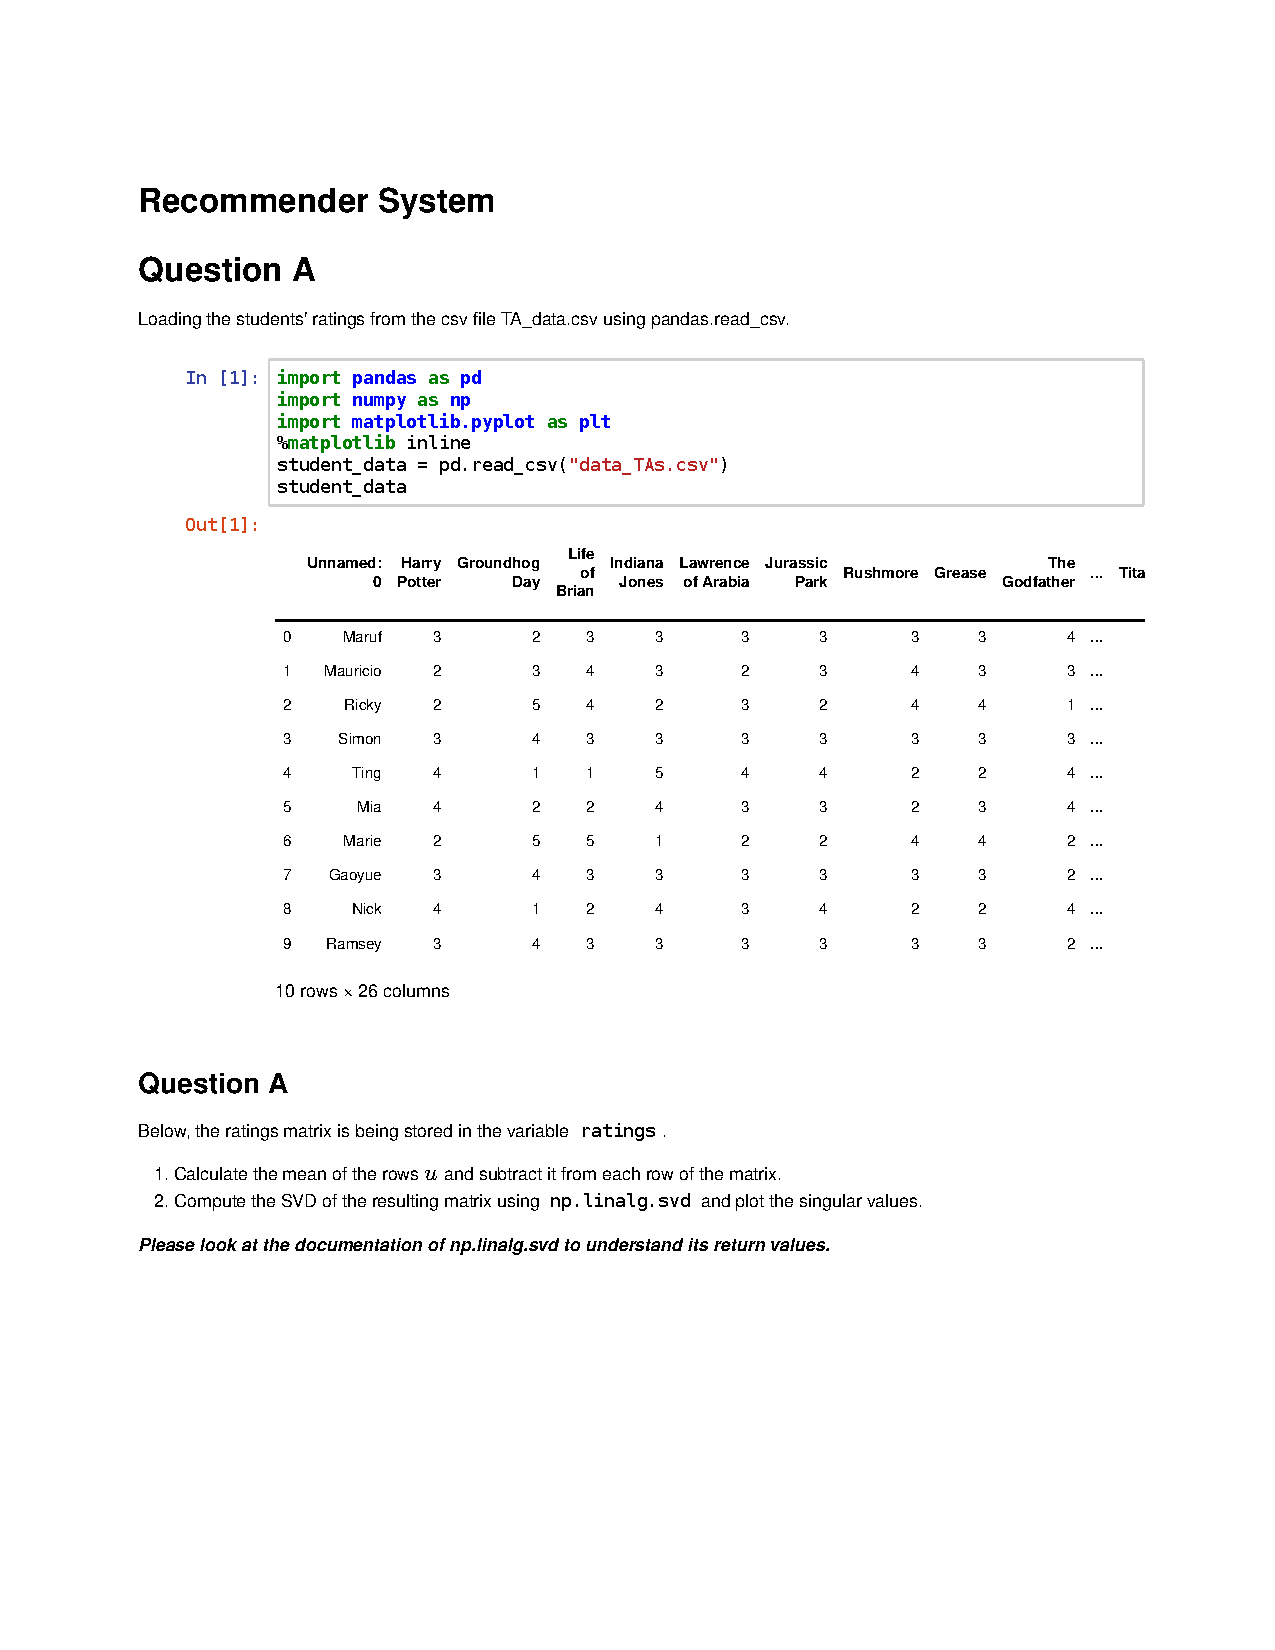
\includepdf[pages=-]{recommender_system.pdf}

\end{document}
